% !TeX spellcheck = en_US
% !TeX encoding = utf8
% !TeX program = xelatex
% !BIB program = bibtex

\documentclass[notes]{beamer}

%\usepackage{pgfpages}
%\setbeameroption{show notes on second screen}

\usepackage[british]{babel}
\usepackage{graphicx,hyperref,ru,url}
% \usepackage{hanging}

\usepackage{listings}
\usepackage{fontspec}
\usefonttheme[onlymath]{serif}
\usepackage{xeCJK}
% \usepackage[backend=biber]{biblatex}
% \bibliography{./ref.bib}
%\addbibresource{ref.bib}
\usepackage{indentfirst}
\usepackage{longtable}
\usepackage{graphicx}
\usepackage{float}
%\usepackage{picins}
\usepackage{rotating}
\usepackage{subfigure}
\usepackage{tabu}
\usepackage{amsmath}
\usepackage{amssymb}
\usepackage{setspace}
\usepackage{amsfonts}
\usepackage{appendix}
\usepackage{listings}
\usepackage{xcolor}
\usepackage{geometry}
\setCJKfamilyfont{cjkhwxk}{SimSun}
\newcommand*{\cjkhwxk}{\CJKfamily{cjkhwxk}}
%\newfontfamily{\consolas}{Consolas}
%\newfontfamily{\monaco}{Monaco}
%\setmonofont[Mapping={}]{Consolas}	%英文引号之类的正常显示,相当于设置英文字体
%\setsansfont{Consolas} %设置英文字体 Monaco, Consolas,  Fantasque Sans Mono
\setmainfont{Times New Roman}
\newfontfamily{\consolas}{Times New Roman}
\newfontfamily{\monaco}{Arial}
\setCJKmainfont{Times New Roman}
%\setmainfont{MONACO.TTF}
%\setsansfont{MONACO.TTF}
\newcommand{\verylarge}{\fontsize{60pt}{\baselineskip}\selectfont}  
\newcommand{\chuhao}{\fontsize{44.9pt}{\baselineskip}\selectfont}  
\newcommand{\xiaochu}{\fontsize{38.5pt}{\baselineskip}\selectfont}  
\newcommand{\yihao}{\fontsize{27.8pt}{\baselineskip}\selectfont}  
\newcommand{\xiaoyi}{\fontsize{25.7pt}{\baselineskip}\selectfont}  
\newcommand{\erhao}{\fontsize{23.5pt}{\baselineskip}\selectfont}  
\newcommand{\xiaoerhao}{\fontsize{19.3pt}{\baselineskip}\selectfont} 
\newcommand{\sihao}{\fontsize{14pt}{\baselineskip}\selectfont}      % 字号设置  
\newcommand{\xiaosihao}{\fontsize{12pt}{\baselineskip}\selectfont}  % 字号设置  
\newcommand{\wuhao}{\fontsize{10.5pt}{\baselineskip}\selectfont}    % 字号设置  
\newcommand{\xiaowuhao}{\fontsize{9pt}{\baselineskip}\selectfont}   % 字号设置  
\newcommand{\liuhao}{\fontsize{7.875pt}{\baselineskip}\selectfont}  % 字号设置  
\newcommand{\qihao}{\fontsize{5.25pt}{\baselineskip}\selectfont}    % 字号设置 

\graphicspath{{./fig/}}

% \setbeamertemplate{footnote}{%
%   \hangpara{2em}{1}%
%   \makebox[2em][l]{\insertfootnotemark}\footnotesize\insertfootnotetext\par%
% }

\definecolor{cred}{rgb}{0.6,0,0}
\definecolor{cgreen}{rgb}{0.25,0.5,0.35}
\definecolor{cpurple}{rgb}{0.5,0,0.35}
\definecolor{cdocblue}{rgb}{0.25,0.35,0.75}
\definecolor{cdark}{rgb}{0.95,1.0,1.0}
\lstset{
	language=R,
	numbers=left,
	numberstyle=\tiny\color{black},
	keywordstyle=\color{cpurple}\consolas,
	commentstyle=\color{cgreen}\consolas,
	stringstyle=\color{cred}\consolas,
	frame=single,
	escapeinside=``,
	xleftmargin=1em,
	xrightmargin=1em, 
	backgroundcolor=\color{cdark},
	aboveskip=1em,
	breaklines=true,
	tabsize=3
} 
% The title of the presentation:
%  - first a short version which is visible at the bottom of each slide;
%  - second the full title shown on the title slide;
\title[Network Performance Prediction]{Evolution Pattern of Statistics \\ though the Training Process of Neural Network}

% Optional: a subtitle to be dispalyed on the title slide
%\subtitle{Show where you're from}

% The author(s) of the presentation:
%  - again first a short version to be displayed at the bottom;
%  - next the full list of authors, which may include contact information;
\author[Summer Intern]{Intern@CUHK}
% The institute:
%  - to start the name of the university as displayed on the top of each slide
%    this can be adjusted such that you can also create a Dutch version
%  - next the institute information as displayed on the title slide

\institute[\wuhao Zhejiang University]{\wuhao\monaco {Information Engineering, ZJU}}

% Add a date and possibly the name of the event to the slides
%  - again first a short version to be shown at the bottom of each slide
%  - second the full date and event name for the title slide
\date[\today]{
   \today}

\begin{document}

\begin{frame}
  \titlepage
\end{frame}

\AtBeginSection[]
{
   \begin{frame}
       \frametitle{Outline}
       \tableofcontents[currentsection]
   \end{frame}
}

\AtBeginSubsection[2-]
{
   \begin{frame}
       \frametitle{Outline}
       \tableofcontents[currentsection]
   \end{frame}
}

\section{Background}
\begin{frame}{Hyper-parameters are not understandable} 
	\begin{block}{SGD Learning Rate}
		\begin{itemize}
			\item Resnet only report its best practice on ImageNet: sgd, init lr = 0.1, decay 10 at epoch 750, 1500.
			\item But using a different hyper parameter suffers from performance degradation.
		\end{itemize}
	\end{block}	
    \begin{figure}
		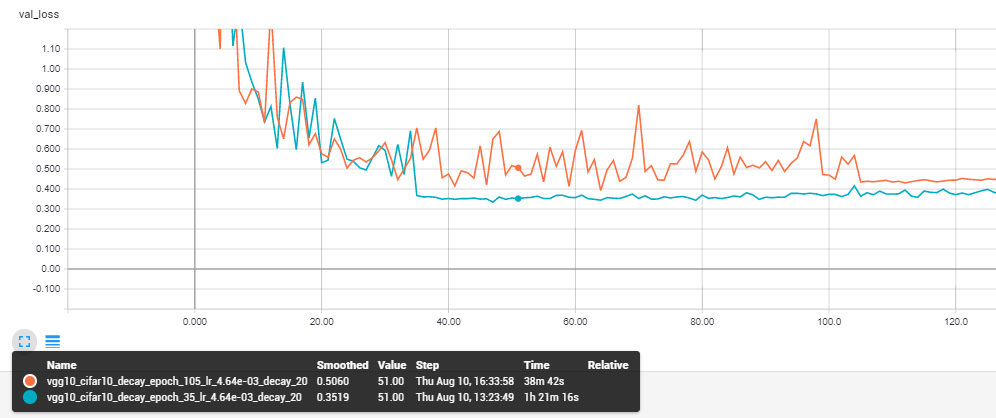
\includegraphics[width=.75\textwidth]{oncifar10.png} \\
        Figure: Similar phenomena on Cifar10 
		\end{figure}
\end{frame}


\begin{frame}{Hyper-parameters are not understandable}
	What is happening inside it?
    \begin{figure}
		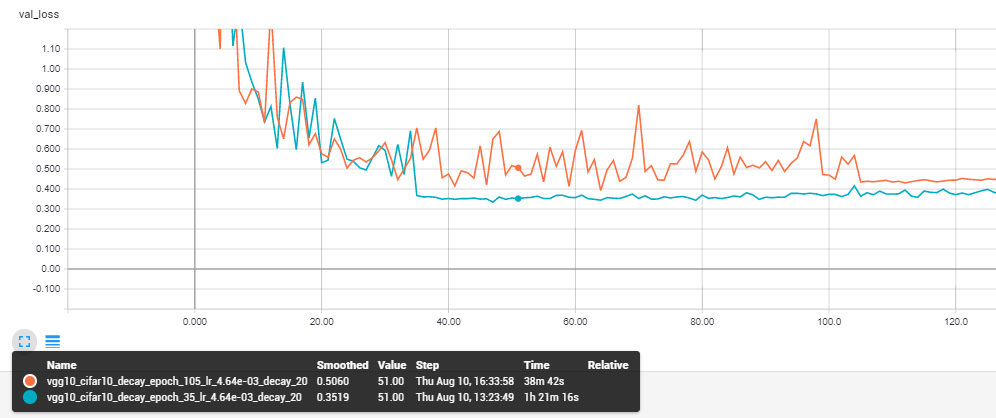
\includegraphics[width=.75\textwidth]{oncifar10.png} \\
        Figure: Similar phenomena on Cifar10 
		\end{figure}
\end{frame} 


\section{Experiments}
\subsection{Sampling}

\begin{frame}{Sample Scheme}
		\begin{longtable}{l||ll}
				\textbf{Log Level} & Spatial Statistics  & Long-term Statistics \\ \hline 
				ALL                  & min/mean/...        & stdtime/diff         \\
				NONF                 & min/mean/...        &                      \\
				SAVE                 &                     &                      \\ \hline \hline 
				\textbf{Log Level} & Short-term Statistics         & Performance          \\ \hline
				ALL                  & loss/val\_acc/...   & loss/val\_acc/...    \\
				NONF                 & loss/val\_acc/...   & loss/val\_acc/...    \\
				SAVE                 & totvar/ptrate(save) &                
		\end{longtable} 
        \liuhao{Spatial Statistics: reduced from one tensor of one timestamp. 
        
        Long-term Statistic: accumulate from the beginning of the training process.
        
        Short-term Statistic: open a windows to observe.
        } 
\end{frame}

\begin{frame}{Sample Scheme}
Calculate statistics sequentially when training at predefined non-fixed sample rate. 
    \begin{figure}
    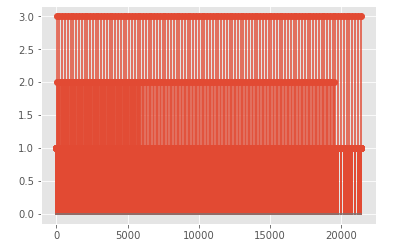
\includegraphics[width=0.33\textwidth]{sample_how.png} 
    \caption{Sample Scheme. Y-axis: ``Log Level'', X-axis: ``iter''}
    \end{figure}
   \textit{e.g.}
   $$f= \left\{ 
       \begin{array}{lll} 4/T_{e} &, t < 30T_{e} & \text{Main Sample Rate} \\ 2/T_{e} &,t < 100T_e & \text{Subsample Rate}  \\ 1/T_e &, t \ge 100T_e & \text{Subsample Rate} \end{array}
       \right. $$ 
       ,where  1 epoch  $T_e $ needs 197 iters. 
\end{frame}

\begin{frame}{Sample Problem}
\begin{figure}
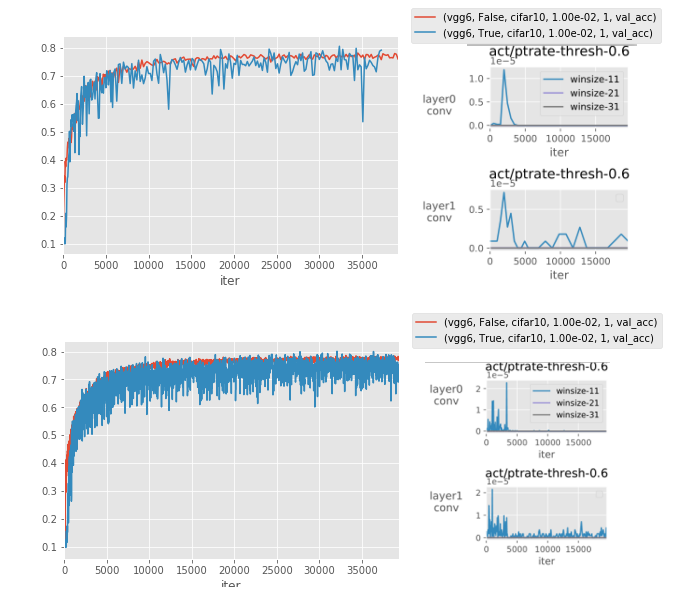
\includegraphics[width=.75\textwidth]{sample_prob.png}
\end{figure}
\note{Note that Suddenly change in sparse sample may because:

- Noise from stochastic batch + sparse sampling

- Some rare event does happen
}
\end{frame}

% \begin{frame}{Consideration}
% 	Disk, Memory, Speed, Information
% 	\begin{itemize}
% 		\item<1-> Disk: To save all weights consumes a lot, with no benefits. 
% %         \note{- load slowly - redundant for training a meta model)}
% 		\item<1-> Memory: Occupy 12*4 GB when training now. 
% %         \note{sequentially calc statistics}
% 		\item<2-> Information: 
% 		\begin{enumerate}
% 			\item<2->   Visualize: resample v.s. artifacts 
% 			\only<2>{\begin{figure}
% 					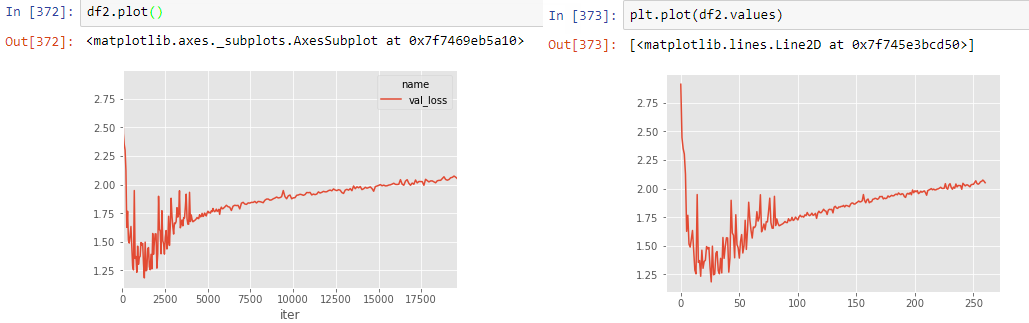
\includegraphics[width=0.5\textwidth]{sample_rate_impact.png}
% 			\end{figure}  }
% 			\item<3->   Impact: Discover some rare event v.s. Smooth
% 			 \only<3>{	
% 				\begin{figure}
% 					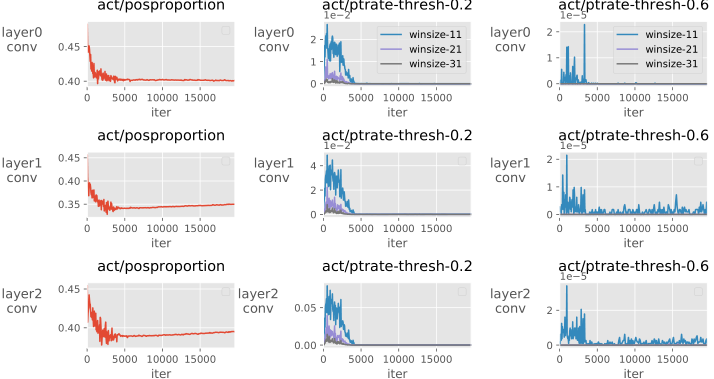
\includegraphics[width=0.75\textwidth]{impact_sparse.png}
% 			\end{figure}}
% 			\uncover<4>{
% 			\begin{figure}
% 				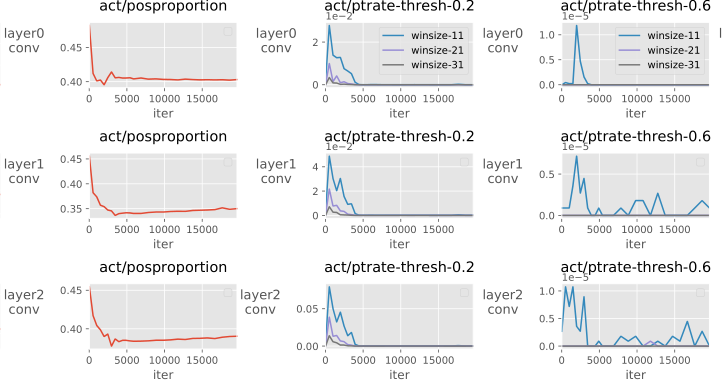
\includegraphics[width=0.75\textwidth]{impact_dense.png}
% 		\end{figure}  }
% 		\end{enumerate}
% 	\end{itemize}
% \end{frame}	

\subsection{Statistics}
% \begin{frame}{Observation}
% Class of Statistics: Apart from shared statistics(\textit{mean/orthogonality/diff/totvar/...}), Activation and Kernel have some exclusive statistics. 
% \begin{longtable}{l||llll}
% \textbf{Parameter}                & Spatial Statistics     & Long-time Statistics \\ \hline
% Activation, \textit{i.e.} Outputs & \alert{+orthogonality}  &                      \\
% Kernel,\textit{i.e.} Weight       & \alert{+orthogonality} &                      \\
% Bias                              &                        &                      \\ \hline\hline
% \textbf{Parameter}                & Short-time Statistics  &                      \\ \hline
% Activation, \textit{i.e.} Outputs & \alert{+ptrate}        &                      \\
% Kernel,\textit{i.e.} Weight       &                        &                      \\ 
% Bias                             & & 
% \end{longtable}
% \note{1. Activation aka. Layer Output aka. Layer Responses \\ }
% \note{2. All stat: 'diff', 'stdtime', 'iqr', 'std', 'mean', 'median', 'magmean', 'posmean', 'negmean', 'posproportion', \\
%                   'max', 'min', 'orthogonality', 'sparsity', 'ptrate-thresh-0.2', 'ptrate-thresh-0.6', \\
%                   'ptrate-thresh-mean', 'totvar'}
% \end{frame}

% \begin{frame}{Performance Curve }
% Analyze \textit{resnet10/cifar10/1.00e\-03} \&  \textit{vgg10/cifar10/1.00e\-02} (Best lr for each model, converge well)
% \begin{figure}
% 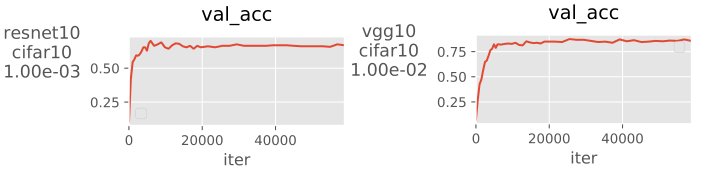
\includegraphics[width= .85\linewidth]{val_acc.png}
% \end{figure}
% \end{frame}

\begin{frame}{Preface}
Some words before studying statistical pattern interactively:
 \begin{itemize}
 \item Activation = Output of one layer. 
 \item Activation and kernel statistical pattern share some similarity.
 \item Conv and FC layer is quite different. 
 \item The architecture is updated to soa, with BN, DP, and Preactive. 
 \item Layer is counted by number of conv.
 \end{itemize}
\end{frame}


\begin{frame}{Stdtime} 	
Aka. \emph{Square Root of 2nd Moment along the time}. 

Make sure equal time interval by calculating at  each \alert{main sample point}.
% For each output of  neural, to calculate std along the time(\textit{stdtime}) at each \alert{main sample point} {\qihao{(Thus, time interval is equal)}}

% , we need sequentially update it: 			 
% $$ \begin{array}{ll} 
% M_{2,n} &   \approx M_{2,n-1} + (x_n - \bar x_{n-1})(x_n - \bar x_n) \\
%  s_{n}^{2}& \approx {\frac {M_{2,n}}{n-1}}
% \end{array}$$
% ,where $ {\displaystyle M_{2,n}} M_{2,n}$ maintains the ssd error relative to current mean. 
\begin{itemize}
\item Measure active of a layer throughout the training time. 
\item Converge to a constant, as NN cooling down.
\item Some conclusion \begin{enumerate}
\item Little activations undergo massive changes.
\item Active individual at the beginning may not active at all training phase of NN. 
\item Activest individuals have similar trending and evolve pattern. 
\item There is some sudden change of value of individual. 
\end{enumerate}
\end{itemize}
\end{frame}

\begin{frame}{Stdtime}
Evidence: 

\begin{minipage}{0.49\textwidth}
\centering
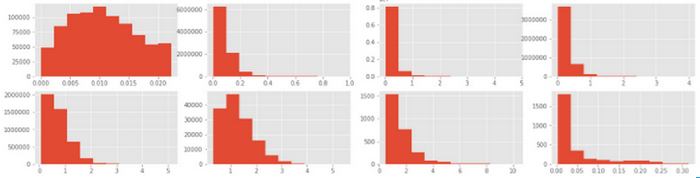
\includegraphics[width=.95\textwidth]{stdtime_dist.png}\\
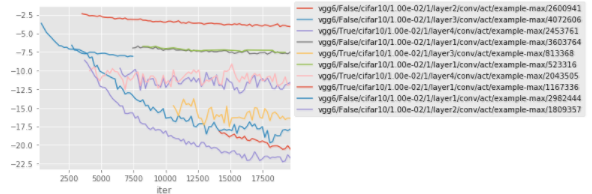
\includegraphics[width=.95\textwidth]{stdtime_incon.png}

\end{minipage}
\begin{minipage}{0.49\textwidth}
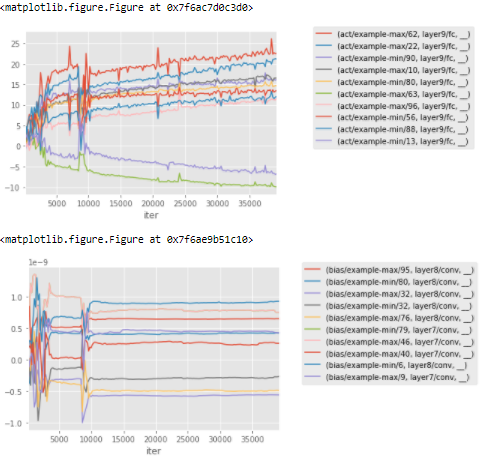
\includegraphics[width=.95\textwidth]{stdtime_sim.png}
\end{minipage}
\end{frame}

\begin{frame}{IQR/Std}
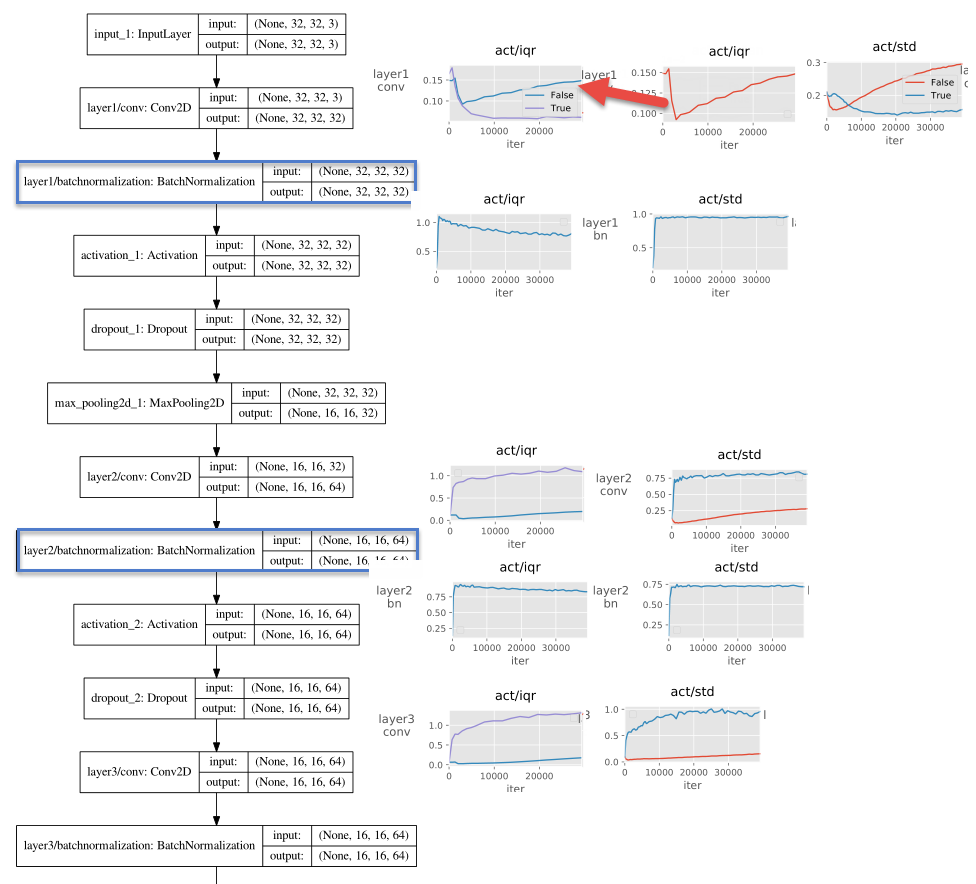
\includegraphics[width=\textwidth]{vgg_bn.png}
\end{frame}
\begin{frame}{IQR/Std}
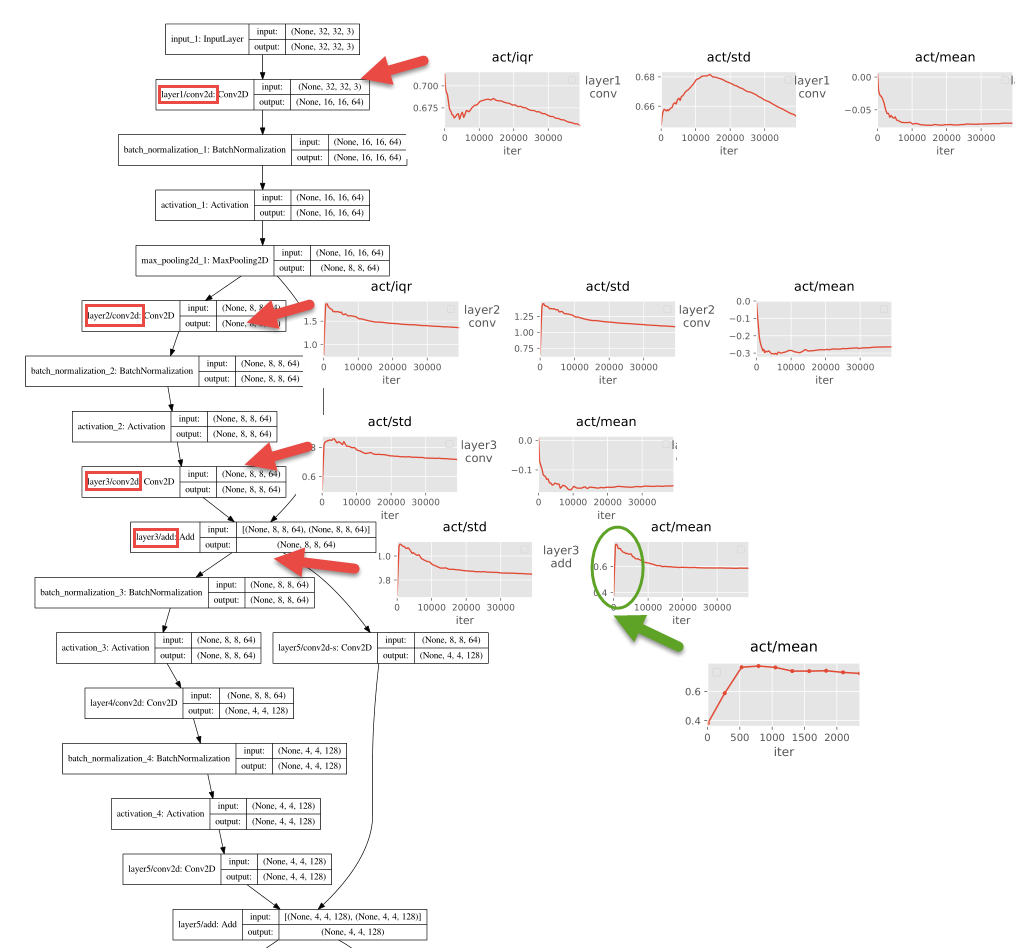
\includegraphics[width=\textwidth]{resnet_bn.png}
\end{frame}

\note{
iqr/std: Behave approximately same. Exception: iqr  takes $1$ in onehot vector as outlier.

std of Resnet10  increases then \alert{decreases} while vgg10 std increase stably. This is explained in {\color{brown}{\href{https://arxiv.org/pdf/1512.03385.pdf}{Resnet Paper}} }: ``residual functions might be generally closer to zero than the non-residual functions''.

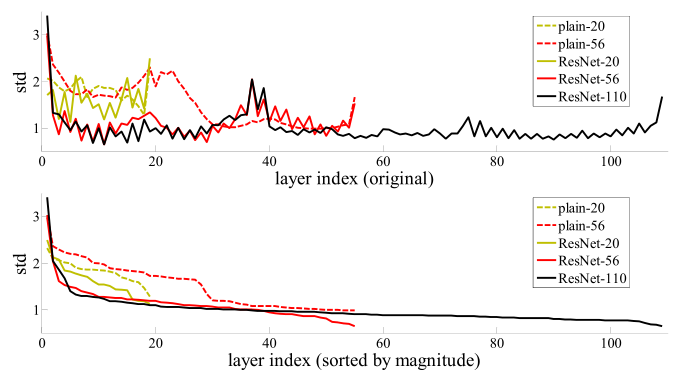
\includegraphics[width=.75\textwidth]{resnet_paper.png}
}


\begin{frame}{Sparsity}
\begin{block}{Definition}
The proportion of value smaller than $0.1\times\text{Mean}$. Only work for distribution with Mean = 0. 
\end{block}

\begin{itemize}
\item Activation/Kernel: \begin{itemize}
\item Shared trending: Increase steadily.
\item Both for Vgg \& ResNet! 
\item Question: Which distribution satisfying: Sparsity $\uparrow$, while Std $\uparrow$
\end{itemize}
\item Bias: No trending.  Mean($10^{-9}$), Std($10^{-8}$). 
\end{itemize}
\end{frame}


\begin{frame}{Orthogonality}
% 	\begin{block}{Dimension} 
% 		\liuhao 
%         - conv kernel: (3,3,3,128)  (filter\_height,filter\_width,in\_channels, out\_channels)
		
% 		- conv act: (272,8,8,256) (batch\_size,img\_height,img\_width,channels)
		
% 		- fc kernel: (256,10) (size\_in,size\_out)
		
% 		- fc act: (272,2048) (batch\_size,channels)
% 	\end{block}
	\begin{example}
    \wuhao 
    \begin{itemize}
    \item between sample: reshape as (272,16384),   calc. between 272 vectors.
    \item between feature map: reshape as (17408,256), calc. between 256 vectors.  
    \item between each placeholder: reshape as (272,16384), calc. between 16384 vectors.
    \end{itemize}
	\end{example}
\end{frame}

\begin{frame}{Polarity Transition Rate (\textit{aka.} ptrate)}
For the figures, Ref. to ``2\_Statistics along training process''.
	\begin{block}{Comments} 
		\begin{itemize}
		\item   ``thresh=0.6, winsize=11'' discover some rare events. 
		\item  ``mean,  winsize=11'' measure the activity level of a layer stably. 
		\item Due to back-propagation, output(bottom in figure, index 10) layer gets to active first then propagate to input layer(top in figure, index 0). 
        \item Resnet is more active and protected from Gradient Vanishing.
		\end{itemize} 
	\end{block} 
\end{frame}

\begin{frame}{Polarity Transition Rate (\textit{aka.} ptrate)}
\begin{figure} 
		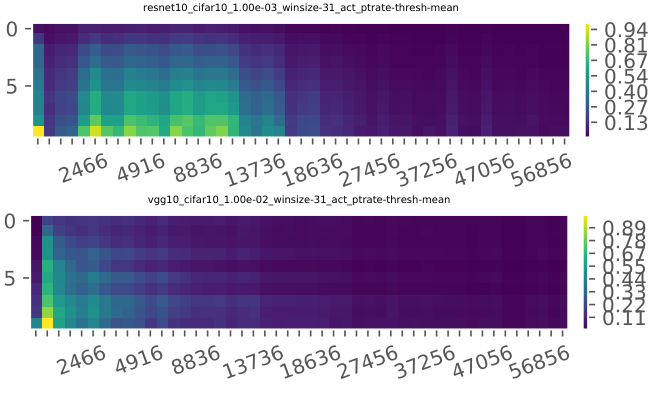
\includegraphics[width=.75\textwidth]{heatmap.png}
	\end{figure}
\end{frame}

\begin{frame}{Other Statistics}
\begin{description}
\item[UpdateRatio] $\frac{ \mathit{mean}(|W_{i+1} - W_{i}|)}{\mathit{mean} (|W_{i}|)}$  

% \text{Mean Magnitude of Difference}}{\text{Mean Magnitude of Last Time Tensor}
It is said as a rule of thumb to select lr: this ratio for kernel weights should be around 1:1000 = 0.001. 
% Note that is a rough guide only, and may not be appropriate for all networks. 
\item[Histogram] Conserve most information, including  Kurtosis, Skewness.
\end{description}
\end{frame}


\section{TODO}
\begin{frame}{TODO}
\begin{itemize}
\item ICLR paper of recent three years
\item {\color{brown}\url{https://github.com/luzai/Perf_Pred/invitations}}
\item ImageNet + lr scheme
\end{itemize}
\end{frame}

%\begin{frame}[t, allowframebreaks]
%\frametitle{References}
%
%
%\printbibliography
%\end{frame}
\begin{frame}
\chuhao Thank you! %\fontspec{LHANDW.TTF}
\end{frame}
		
	
\end{document} 